\section{mo\-Rand\-Impr\-Select$<$ M $>$ Class Template Reference}
\label{classmo_rand_impr_select}\index{moRandImprSelect@{moRandImprSelect}}
One of the possible {\bf mo\-Move}{\rm (p.\,\pageref{classmo_move})} selector ({\bf mo\-Move\-Select}{\rm (p.\,\pageref{classmo_move_select})}).  


{\tt \#include $<$mo\-Rand\-Impr\-Select.h$>$}

Inheritance diagram for mo\-Rand\-Impr\-Select$<$ M $>$::\begin{figure}[H]
\begin{center}
\leavevmode
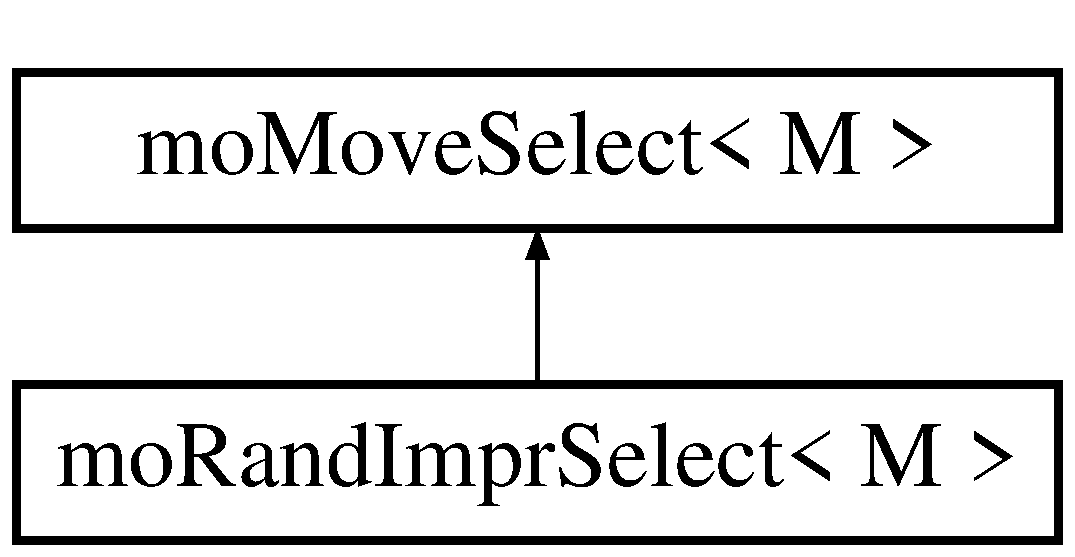
\includegraphics[height=4cm]{classmo_rand_impr_select}
\end{center}
\end{figure}
\subsection*{Public Types}
\begin{CompactItemize}
\item 
typedef M::EOType::Fitness {\bf Fitness}\label{classmo_rand_impr_select_w0}

\begin{CompactList}\small\item\em Alias for the fitness. \item\end{CompactList}\end{CompactItemize}
\subsection*{Public Member Functions}
\begin{CompactItemize}
\item 
void {\bf init} (const {\bf Fitness} \&\_\-fitness)
\begin{CompactList}\small\item\em Procedure which all that needs a mo\-Rand\-Impr\-Select. \item\end{CompactList}\item 
bool {\bf update} (const M \&\_\-move, const {\bf Fitness} \&\_\-fitness)
\begin{CompactList}\small\item\em Function that updates the fitness and move vectors. \item\end{CompactList}\item 
void {\bf operator()} (M \&\_\-move, {\bf Fitness} \&\_\-fitness)
\begin{CompactList}\small\item\em The move selection. \item\end{CompactList}\end{CompactItemize}
\subsection*{Private Attributes}
\begin{CompactItemize}
\item 
{\bf Fitness} {\bf initial\_\-fitness}\label{classmo_rand_impr_select_r0}

\begin{CompactList}\small\item\em Fitness of the current solution. \item\end{CompactList}\item 
std::vector$<$ {\bf Fitness} $>$ {\bf better\_\-fitnesses}\label{classmo_rand_impr_select_r1}

\begin{CompactList}\small\item\em Candidate fitnesse vector. \item\end{CompactList}\item 
std::vector$<$ M $>$ {\bf better\_\-moves}\label{classmo_rand_impr_select_r2}

\begin{CompactList}\small\item\em Candidate move vector. \item\end{CompactList}\item 
bool {\bf first\-Time}\label{classmo_rand_impr_select_r3}

\begin{CompactList}\small\item\em Indicate if update has been called or not. \item\end{CompactList}\end{CompactItemize}


\subsection{Detailed Description}
\subsubsection*{template$<$class M$>$ class mo\-Rand\-Impr\-Select$<$ M $>$}

One of the possible {\bf mo\-Move}{\rm (p.\,\pageref{classmo_move})} selector ({\bf mo\-Move\-Select}{\rm (p.\,\pageref{classmo_move_select})}). 

All the neighbors are considered. One of them that enables an improvment of the objective function is choosen. 



Definition at line 49 of file mo\-Rand\-Impr\-Select.h.

\subsection{Member Function Documentation}
\index{moRandImprSelect@{mo\-Rand\-Impr\-Select}!init@{init}}
\index{init@{init}!moRandImprSelect@{mo\-Rand\-Impr\-Select}}
\subsubsection{\setlength{\rightskip}{0pt plus 5cm}template$<$class M$>$ void {\bf mo\-Rand\-Impr\-Select}$<$ M $>$::init (const {\bf Fitness} \& {\em \_\-fitness})\hspace{0.3cm}{\tt  [inline, virtual]}}\label{classmo_rand_impr_select_a0}


Procedure which all that needs a mo\-Rand\-Impr\-Select. 

Give a value to the initialise fitness. Clean the move and fitness vectors.

\begin{Desc}
\item[Parameters:]
\begin{description}
\item[{\em \_\-fitness}]the current best fitness \end{description}
\end{Desc}


Implements {\bf mo\-Move\-Select$<$ M $>$} {\rm (p.\,\pageref{classmo_move_select_a0})}.

Definition at line 63 of file mo\-Rand\-Impr\-Select.h.

References mo\-Rand\-Impr\-Select$<$ M $>$::better\_\-fitnesses, mo\-Rand\-Impr\-Select$<$ M $>$::better\_\-moves, mo\-Rand\-Impr\-Select$<$ M $>$::first\-Time, and mo\-Rand\-Impr\-Select$<$ M $>$::initial\_\-fitness.\index{moRandImprSelect@{mo\-Rand\-Impr\-Select}!update@{update}}
\index{update@{update}!moRandImprSelect@{mo\-Rand\-Impr\-Select}}
\subsubsection{\setlength{\rightskip}{0pt plus 5cm}template$<$class M$>$ bool {\bf mo\-Rand\-Impr\-Select}$<$ M $>$::update (const M \& {\em \_\-move}, const {\bf Fitness} \& {\em \_\-fitness})\hspace{0.3cm}{\tt  [inline, virtual]}}\label{classmo_rand_impr_select_a1}


Function that updates the fitness and move vectors. 

if a move give a better fitness than the initial fitness, it is saved and the fitness too.

\begin{Desc}
\item[Parameters:]
\begin{description}
\item[{\em \_\-move}]a new move. \item[{\em \_\-fitness}]a new fitness associated to the new move. \end{description}
\end{Desc}
\begin{Desc}
\item[Returns:]true. \end{Desc}


Implements {\bf mo\-Move\-Select$<$ M $>$} {\rm (p.\,\pageref{classmo_move_select_a1})}.

Definition at line 80 of file mo\-Rand\-Impr\-Select.h.

References mo\-Rand\-Impr\-Select$<$ M $>$::better\_\-fitnesses, mo\-Rand\-Impr\-Select$<$ M $>$::better\_\-moves, and mo\-Rand\-Impr\-Select$<$ M $>$::first\-Time.\index{moRandImprSelect@{mo\-Rand\-Impr\-Select}!operator()@{operator()}}
\index{operator()@{operator()}!moRandImprSelect@{mo\-Rand\-Impr\-Select}}
\subsubsection{\setlength{\rightskip}{0pt plus 5cm}template$<$class M$>$ void {\bf mo\-Rand\-Impr\-Select}$<$ M $>$::operator() (M \& {\em \_\-move}, {\bf Fitness} \& {\em \_\-fitness})\hspace{0.3cm}{\tt  [inline]}}\label{classmo_rand_impr_select_a2}


The move selection. 

One the saved move is randomly chosen.

\begin{Desc}
\item[Parameters:]
\begin{description}
\item[{\em \_\-move}]the reference of the move that can be initialised by the function. \item[{\em \_\-fitness}]the reference of the fitness that can be initialised by the function. \end{description}
\end{Desc}


Definition at line 100 of file mo\-Rand\-Impr\-Select.h.

References mo\-Rand\-Impr\-Select$<$ M $>$::better\_\-fitnesses, and mo\-Rand\-Impr\-Select$<$ M $>$::better\_\-moves.

The documentation for this class was generated from the following file:\begin{CompactItemize}
\item 
mo\-Rand\-Impr\-Select.h\end{CompactItemize}
